\documentclass{article}
\usepackage{algorithm2e}
\usepackage{amsmath}
\usepackage{amssymb}
\usepackage{amstext}
\usepackage{color}
\usepackage{enumerate}
\usepackage{fancyvrb}
\usepackage{framed}
\usepackage{fullpage}
\usepackage{graphicx}
\usepackage{xspace}

% Logical operators
\def\NOT{\neg}
\def\AND{\wedge}
\def\OR{\vee}
\def\XOR{\otimes}
\def\IMP{\Rightarrow}
\def\BIMP{\Leftarrow}
\def\IFF{\Leftrightarrow}
\def\LIFF{\hspace{1em}\Longleftrightarrow\hspace{1em}}
\def\TRUE{\ensuremath\mathtt{true}}
\def\FALSE{\ensuremath\mathtt{false}}

% Layout
\def\anchor{\hspace{0em}\vspace*{-1.25em}\\}
\def\return{\hspace{0em}\\}

% Environments
\DefineVerbatimEnvironment{alg}{Verbatim}{frame=single,commandchars=\\\{\},codes={\catcode`$=3\catcode`^=7}}
\DefineVerbatimEnvironment{code}{Verbatim}{frame=single}

% Shortcuts
\def\field#1{\mathbb{#1}}
\def\prm{^\prime}
\def\<{\langle}
\def\>{\rangle}
\def\nil{\varnothing}
\def\G{{\sf Greedy}\xspace}
\def\O{{\sf OPT}\xspace}

% Calculus shortcuts
\def\eps{\epsilon}
\def\vare{\varepsilon}
\def\dx{\; dx \;}

% Style tweaks
\setlength{\jot}{1em}

\begin{document}


\noindent
\begin{center}
  \framebox {
    \vbox {
      \hbox to 6.28in {\bf  Math 275: Statistical Inference \hfill Winter 2014}
      \hbox to 6.28in {\it Homework \#7 \hfill Calder Coalson}}}
\end{center}\vspace{0em}


\section*{Chapter 6}
\begin{enumerate}


\item[28.]
\begin{align}
	\hat\theta_1\prm &= \dfrac{\hat\theta_1}{0.9}
	& E[\hat\theta_1\prm] &= \dfrac{E[\hat\theta_1]}{0.9} = \theta
	& V[\hat\theta_1\prm] &= \dfrac{V[\hat\theta_1]}{0.9^2} = 3.70
	\notag\\
	\hat\theta_2\prm &= \dfrac{\hat\theta_2}{1.2}
	& E[\hat\theta_2\prm] &= \dfrac{E[\hat\theta_2]}{1.2} = \theta
	& V[\hat\theta_2\prm] &= \dfrac{V[\hat\theta_2]}{1.2^2} = 1.39
	\notag
\end{align}

$V[\hat\theta_2\prm] < V[\hat\theta_1\prm]$ so $\hat\theta_2\prm$ is more efficient.


\item[29.]
\begin{align}
	E[\hat\theta_1]
		&= E[X_1]
		= \int_0^\infty x \dfrac{e^{-x/\theta}}{\theta} \dx
		= \theta
	& V[\hat\theta_1]
		&= V[X_1]
		= \int_0^\infty x^2 \dfrac{e^{-x/\theta}}{\theta} \dx
		= 2 \theta^2
	\notag\\
	E[\hat\theta_2]
		&= E\left[\dfrac{X_1 + X_2}{2}\right]
		= \dfrac{E[X_1] + E[X_2]}{2}
		= \theta
	&\hspace{2em} V[\hat\theta_2]
		&= V\left[\dfrac{X_1 + X_2}{2}\right]
		= \dfrac{V[X_1] + V[X_2]}{4}
		= \theta^2
	\notag\\
	E[\hat\theta_3]
		&= E\left[\dfrac{X_1 + 2X_2}{3}\right]
		= \dfrac{E[X_1] + 2E[X_2]}{3}
		= \theta
	&\hspace{2em} V[\hat\theta_3]
		&= V\left[\dfrac{X_1 + 2X_2}{3}\right]
		= \dfrac{V[X_1] + 4V[X_2]}{9}
		= \dfrac{10}{9} \theta^2
	\notag
\end{align}


\item[30.]
\begin{enumerate}
\item
\begin{align}
	MSE[\hat\theta_1] &= B[\hat\theta_1]^2 + V[\hat\theta_1] = 0^2 + 25 = 25
	\notag\\
	MSE[\hat\theta_2] &= B[\hat\theta_2]^2 + V[\hat\theta_2] = 3^2 + 4 = 13
	\notag
\end{align}

\item
\begin{align}
	MSE[\hat\theta_2] &< MSE[\hat\theta_1]
	\notag\\
	b^2 + 4 &< 25
	\notag\\
	b &< \sqrt{19}
	\notag
\end{align}
\end{enumerate}


\newpage
\item[31.]\hspace{0em}\\
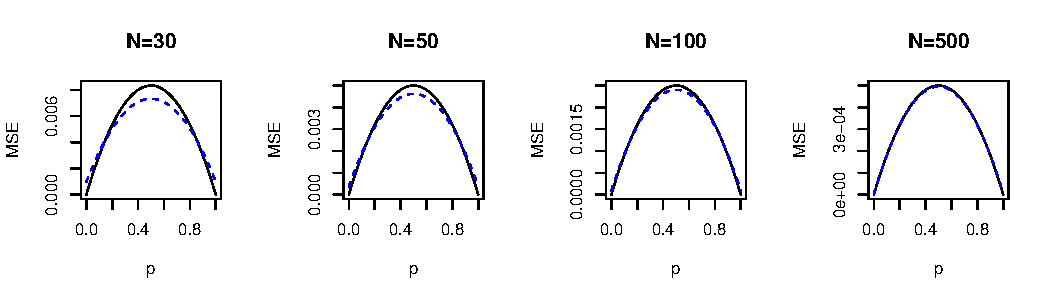
\includegraphics[width=0.98\textwidth]{6-31.pdf}
\begin{code}
f = function (n) {
  curve(x*(1-x)/n, from=0, to=1, main=sprintf("N=%d",n), xlab="p", ylab="MSE")
  curve(n * (1-x)*x/(n+2)^2 + (1-2*x)^2/(n+2)^2, add=TRUE, col="blue", lty=2)
}
f(30); f(50); f(100); f(200)
\end{code}
The MSE converges on the MSE of the original estimator as $N \rightarrow \infty$.


\item[32.]
\begin{enumerate}
\item
\begin{align}
	B[\hat\beta_1] &= E[\hat\beta_1] - \beta \notag\\
	&= (n+1) E[X_{min}] - \beta \notag\\
	&= (n+1) \int_0^\beta x \dfrac{1}{\beta} \left(\dfrac{x}{\beta}\right)^{n-1} dx - \beta \notag\\
	&= (n+1) \dfrac{1}{\beta^n} \int_0^\beta x^n dx - \beta \notag\\
	&= (n+1) \dfrac{\beta}{n+1} - \beta \notag\\
	&= 0 \notag
\end{align}

\item
\begin{align}
	\dfrac{V[\hat\beta_1]}{V[\hat\beta_2]}
	&= \dfrac{V[(n+1)X_{min}]}{V[((n+1)/n)X_{max}]}
	\notag\\
	&= n^2 \dfrac{V[X_{min}]}{V[X_{max}]}
	\notag\\
	&= n^2 \dfrac{V[X_{min}]}{V[X_{min}]}
	\tag{\text{by symmetry}}
	\notag\\
	&= n^2
	\notag
\end{align}
\end{enumerate}


\newpage
\item[33.]
\begin{enumerate}
\item
\begin{align}
	E[X_i] &= \int_0^{1/\theta} x 2 \theta^2 x \dx = \dfrac{2}{3 \theta} \notag
\end{align}

\item
\begin{align}
	B[T] &= E[T] - \dfrac{1}{\theta}
	&\hspace{4em} MSE[T] &= B[T]^2 + V[T]
	\notag\\
	&= \dfrac{E[X_i]}{9} + \dfrac{E[X_i]}{9} + \dfrac{E[X_i]}{3} - \dfrac{1}{\theta}
	&&= \dfrac{17^2}{27^2 \theta^2} + \int_0^{1/\theta} x^2 2 \theta^2 x \dx
	\notag\\
	&= \dfrac{10}{27 \theta} - \dfrac{1}{\theta}
	&&= \dfrac{17^2}{27^2 \theta^2} + \dfrac{1}{2 \theta^2}
	\notag\\
	&= -\dfrac{17}{27 \theta}
	&&= \dfrac{1307}{1458 \theta^2}
	\notag
\end{align}

\item
Let $T\prm = \frac{27}{10} T$.
\begin{align}
	B[T\prm] &= E[T\prm] - \dfrac{1}{\theta}
	\notag\\
	&= \dfrac{27}{10} E[T] - \dfrac{1}{\theta}
	\notag\\
	&= 0
	\notag
\end{align}
\end{enumerate}


\end{enumerate}
\section*{Chapter 7}
\begin{enumerate}


\item[1.]


\item[2.]


\item[3.]


\item[5.]


\end{enumerate}


\end{document}